\chapter{Multivariate component-wise boosting on survival data}
In this chapter, we propose a component-wise boosting algorithm for fitting the inverse gaussian first hitting time model to survival data.

\section{Simulation of survival data}
We wish to simulate survival times $\ti,i=1,\ldots,N$ with censoring. We first draw survival times $\tilde{t}_i$ from some survival time distribution $f(\cdot)$. If this distribution has a closed form probability distribution function, we can draw from it directly. If not, we might use some an inverse sampling method, e.g. by drawing unit exponentials and using a corresponding transformation.

To censor the data, we draw censoring times $W_i\sim f(\cdot),i=1,\ldots,N$, from a more right-tailed distribution, meaning we want to get many, but not all, $W_i$'s to be larger than the $\tilde{t}_i$'s. We let the observed survival times then be $t_i=\min(\tilde{t}_i,W_i)$.
The corresponding observed indicator, $\di$, is then set equal to 1 if the actual survival time was observed, i.e., if $\ti<W_i$. We end up with a set of $N$ tuples $(t_i,\delta_i),i=1,\ldots,N$. Note that this scheme incorporates independent censoring: The censoring time is independent of the survival times.

\begin{algorithm}
\caption{Generating survival data from Inverse Gaussian FHT distribution}
\label{algo:FHT-sim}
\begin{enumerate}
    \item Given design matrices $\X$, $\Z$ and true parameter vectors $\bbeta$ and $\bgamma$.
    \item Link covariates and parameters using link functions
        \begin{align*}
            \ln y_0&=\bbeta^T\X \\
            \mu&=\bgamma^T\Z.
        \end{align*}
    \item Draw $N$ survival times $(t_i)_{i=1}^N$ from IG$(\mu,y_0)$.
    \item Draw a censoring time $W$ from some distribution which is independent of the data.
    \item Right censor data by choosing $\widetilde{t}_i=\min(t_i,W)$. The indicator on whether observation $i$ was observed or not is then $\delta_i=I(\widetilde{t}_i=t_i)$.
    \item The simulated data set is $(\widetilde{t}_i,\delta_i)_{i=1,\ldots,N}$.
\end{enumerate}
\end{algorithm}

\section{Algorithm}
We apply the component-wise boosting algorithm \ref{algo:fhtboost} with loss function $\rho(\mu,\y0)=-\log\loss{y_0,\mu}$. We differentiate the loss function with respect to these two and get .... For more details on the derivation, see \ref{appendix}. \todo{Maybe use $b$ instead of $y_0$, to not get subscript chaos?}

\begin{algorithm}
\caption{FHT Boost with twodimensional loss function}
\label{algo:fhtboost}
\begin{enumerate}
    \item Initialize the $n$-dimensional vectors $\hat{y}_0^{[0]},\hat{\mu}^{[0]}$ with the maximum likelihood estimates as offset values, i.e., $\hat{y}_0^{[0]}, \hat{\mu}^{[0]}=\argmin_{y_0,\mu}\rho(\cdot,\cdot)$.
    \item For both components of the loss function, we specify linear base learners. In particular, a component-wise base learner which can be used for each of the $p$ variables used in $\X$ corresponding to $y_0$ and the $d$ variables in $\Z$ corresponding to $\mu$. Like earlier, the base learner takes one input variable and has one output variable.
    \item Set $m=0$ and $\nu=0.1$.
    \item Increase $m$ by 1.
    \begin{enumerate}
        \item If $m>m_{\text{stop},y_0}$, proceed to step 4 e). If not, compute the negative partial derivative $-\frac{\partial\rho}{\partial y_0}$ and evaluate at $\hat{f}^{[m-1]}(X_i,Z_i)=\left(\hat{y}_0^{[m-1]}(X_i),\hat{\mu}^{[m-1]}(Z_i)\right)_{i=1,\ldots,n}$. This yields the negative gradient vector $U_{y_0}^{[m-1]}=\left(U_{i,y_0}^{[m-1]}\right)_{i=1,\ldots,n}:=\left(-\frac{\partial}{\partial y_0}\rho\left(Y_i,\hat{f}^{[m-1]}(X_i,Z_i)\right)\right)_{i=1,\ldots,n}$.
        \item Fit the negative gradient vector $U_{y_0}^{[m-1]}$ to each of the $p$ components of $\X$ separately (i.e. to each predictor variable) using the base learners specified in step 2. This yields $p$ vectors of predicted values, where each vector is an estimate of the negative gradient vector $U_{y_0}^{[m-1]}$.
        \item Select the component of $\X$ which best fits $U_{y_0}{[m-1]}$ according to $R^2$. Set $\hat{U}_{y_0}^{[m-1]}$ equal to the fitted values of the corresponding best model fitted in the previous step.
        \item Update $\hat{y}_0^{[m-1]}\gets\hat{y}_0^{[m-1]}+\nu\hat{U}_{y_0}^{[m-1]}$.
        \item If $m>m_{\text{stop},\mu}$, proceed to step 4 j). If not, compute the negative partial derivative $-\frac{\partial\rho}{\partial \mu}$ and evaluate at $\hat{f}^{[m-1]}(X_i,Z_i)=\left(\hat{y}_0^{[m-1]}(X_i),\hat{\mu}^{[m-1]}(Z_i)\right)_{i=1,\ldots,n}$. This yields the negative gradient vector $U_{\mu}^{[m-1]}=\left(U_{i,\mu}^{[m-1]}\right)_{i=1,\ldots,n}:=\left(-\frac{\partial}{\partial \mu}\rho\left(Y_i,\hat{f}^{[m-1]}(X_i,Z_i)\right)\right)_{i=1,\ldots,n}$.
        \item Fit the negative gradient vector $U_{\mu}^{[m-1]}$ to each of the $p$ components of $\Z$ separately (i.e. to each predictor variable) using the base learners specified in step 2. This yields $d$ vectors of predicted values, where each vector is an estimate of the negative gradient vector $U_{\mu}^{[m-1]}$.
        \item Select the component of $\Z$ which best fits $U_{\mu}{[m-1]}$ according to $R^2$. Set $\hat{U}_{\mu}^{[m-1]}$ equal to the fitted values of the corresponding best model fitted in the previous step.
        \item Update $\hat{\mu}^{[m-1]}\gets\hat{\mu}^{[m-1]}+\nu\hat{U}_{\mu}^{[m-1]}$.
        \item Update $\hat{f}^{[m]}\gets\hat{f}^{[m-1]}$.
        \item If $m>\max(m_{\text{stop},y_0},m_{\text{stop},\mu})$, go to step 5. If not, repeat step 4.
    \end{enumerate}
    \item Return $\hat{f}^{[m]}$.
\end{enumerate}
\end{algorithm}
We might call this cyclical boosting.

\subsection{Boost in same}
Another way to do this is to only boost one component in each iteration. The component might be corresponding to $X$, or it might be corresponding to $Z$.


% First tried cyclical boosting.
% Then tried non-cyclical, with comparing RSS. Doesn't work; not on the same scale.
% Then tried using non-cyclical, comparing instead the loss function instead of rss.

\subsection{Derivatives not on same scale}
Pass.

\subsection{Changing the intercept in each iteration}
Another way to do this is to only boost one component in each iteration. The component might be corresponding to $X$, or it might be corresponding to $Z$.


\section{Simulation experiments}
In this section, I will discuss how I tried validating the boosting method I have developed. While working with implementing the algorithm, to see if it worked, I first used an example with low dimensions. In low dimensions, it's feasible to find the joint maximum likelihood numerically. After confirming the method works as it should, we can go to more complicated examples.

\section{Simulation setup}
We do simulations where we draw observations from the Inverse Gaussian distribution, i.e., we simulate lifetimes from the first hitting time model with Wiener process as the health process. We use algorithm \eqref{algo:FHT-sim} to do this. We will have two scenarios: One with no correlation, and one with a lot of correlation. To simulate the covariate matrices $X$ and $Z$ we will use algorithm \eqref{algo:clinical-sim}, which is a method for simulating clinical and gene data together. We imagine $X$, corresponding to $\bbeta$, be gene expressions, whereas $Z$, corresponding to $\bgamma$ be clinical measurements. We specify the different correlations for the covariate matrices. But most importantly, we specify the true parameter vectors, $\bbeta$ and $\bgamma$. For each scenario, we conduct $N_{\text{scenario}}$ runs.

One run consists of first drawing data (with a specific seed to ensure reproducibility), i.e., we draw covariate matrices $\X$, $\Z$ from \label{algo:clinical-sim}. $\X$ is of size $N\times p$ and $\Z$ is of size $N\times d$, where $N$ is the number of observations, $p+1$ is the size of the covariate vector $\bbeta$ (including an intercept which will not be affected by the covariates), and $d+1$ is the size of the covariate vector $\bgamma$. Then we combine these with the true covariate matrices to get vectors $\y_0$ and $\mathbf{\mu}$ of initial value of the health process, and drift, respectively. Then we draw from the Inverse Gaussian distribution according to \label{algo:FHT-sim}, obtaining $N$ right-censored lifetimes, i.e., $N$ tuples $(\widetilde{t}_i,\delta_i)_{i=1,\ldots,N}$. With these tuples, then, we can do a run with the FHT boosting algorithm. We first use repeated K-fold cross-validation to find the optimal number of boosting steps, $m_{\text{stop}}$. Then we estimate the model on the whole of this training set. Then we validate this model on a training set of size $N_{\text{test}}$. The data here is drawn in the exact same manner as the training data, here also with a specific seed.

\begin{algorithm}
\caption{Generating clinical and gene expression data}
\label{algo:clinical-sim}
\begin{enumerate}
    \item Lorem ipsum.
\end{enumerate}
\end{algorithm}

\subsection{Small example}
Let parameter vectors be two dense $\bbeta=(2,0.1,0.2)$ and $\bgamma=(-1, -0.1, 0.1)$. Let $X$ and $Z$ be such and such, drawn from a beta distribution.
We simulate data using Algorithm \ref{algo:FHT-sim}, with the censoring time $W$ being drawn from a distribution $\exp(0.1)$. The resulting survival times have the following Kaplan-Meier plot.
\begin{figure}
\caption{Kaplan-Meier plot of small example}
\centering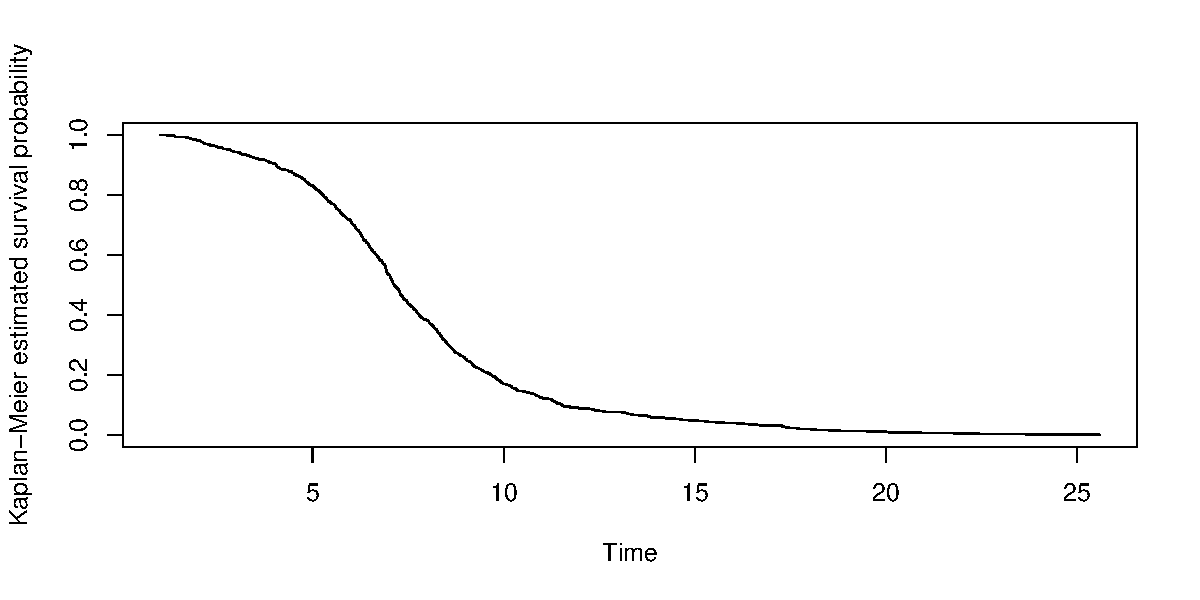
\includegraphics[scale=0.4]{figures/case1.pdf}
\end{figure}
We use cross validation to find a suitable iteration number $\mstop$, and find it to be 28. We then run our algorithm with that number of iterations. Below is a plot of the negative log likelihood of the data (in-sample loss) as a function of iteration number.
\begin{figure}
\caption{Log-likelihood}
\centering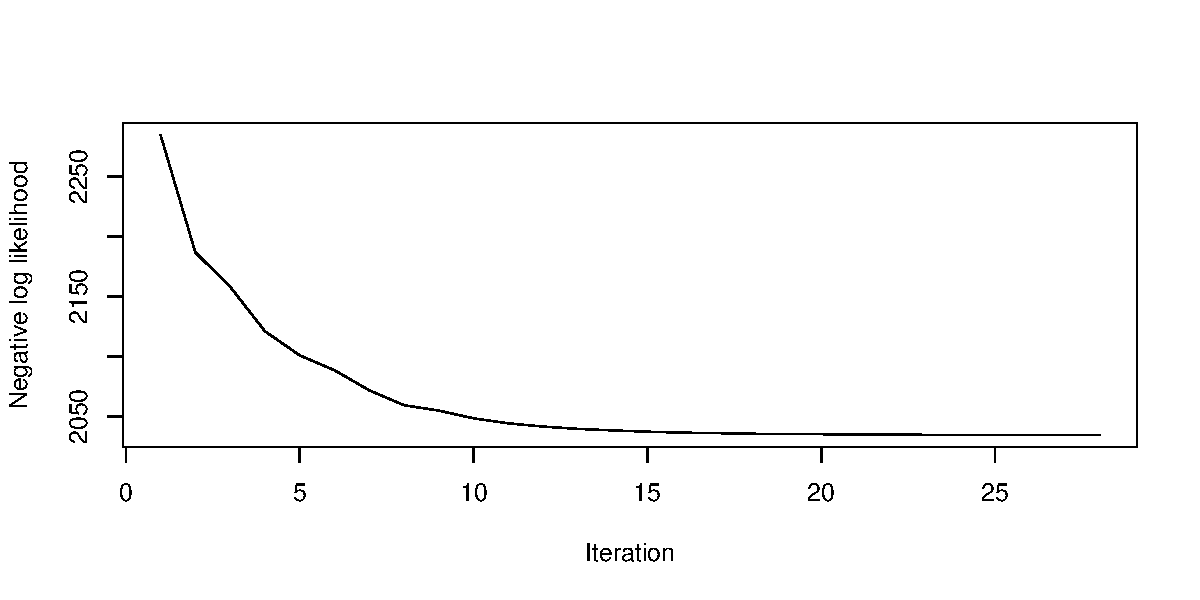
\includegraphics[scale=0.4]{figures/case1_loglik.pdf}
\end{figure}
The final $\hat{\bbeta}$ is $(1.968, 0.103, 0.180)$, and the final $\hat{\bgamma}$ is $(-0.964, -0.082, 0.062)$. The parameters found by numerically maximizing the joint maximum likelihood are also included. Summarized in the table below.

\begin{tabular}{lrr}
    parameter  & true & estimated \\
    $\beta_0$  &  2.0 &     1.968 \\
    $\beta_1$  &  0.1 &     0.103 \\
    $\beta_2$  &  0.2 &     0.180 \\
    $\gamma_0$ & -1.0 &    -0.964 \\
    $\gamma_1$ & -0.1 &    -0.082 \\
    $\gamma_2$ &  0.1 &     0.062 \\
\end{tabular}

As we can see, our boosting method recovers the original parameters quite well. This is of course with data coming from the exact same kind of model.

\section{Brier scores on survival data}
In order to assess predictive performance, we need what's called a proper scoring rule: One which is 1 if the actual data is inserted as predictions.

\subsection{Brier scores and $R^2$ measure}
The Brier score \citep{brier1950} was first introduced as a way to measure the accuracy of weather forecasts. While it is also able to handle multiple categories, we will here give the definition for the binary case. We start by assuming that we are in a situation with no censoring, and that we have $m$ individuals in a test set. We denote their observed survival times by $t_i$, and their covariate vector as $\x_i$, as usual, with $i=1,\ldots,m$. The Brier score aims at evaluating how well the estimated patient specific survival probability $\hat{\pi}(t^*|\x)$, obtained from a prediction model, is able to predict the event status $I(t>t^*)$ of an individual at a given time $t^*$. The error made in predicting the event status $I(t>t^*)$ for a patient in the test set can be given as
\begin{align*}
BS(t^*)&=\frac{1}{M}\sum_{i=1}^m\left(I(t_i>t^*)-\hat{\pi}(t^*|\x_i)\right)^2 \\
    &=\frac{1}{M}\sum_{i=1}^m\left[\hat{\pi}(t^*|\x_i)^2I(t_i\leq t^*)+(1-\hat{\pi}(t^*|\x_i))(I(t_i>t^*)\right].
\end{align*}
In the first formulation, the Brier score looks like a version of an RSS measure, where one sums the squared error between the observed event and the estimated probability. In the case of censored data, the above is of course not enough. The Brier score was adapted to handle censored survival times by \citet{graf}, assuming independent censoring. They showed that the loss of information due to censoring can be accounted for by using an inverse probability of censoring weighting \citep{bovelstadborgan}. This Brier score for censored data is defined as
\begin{equation*}
    BS^c(t^*)=\frac{1}{M}\sum_{i=1}^m\left[\frac{\hat{\pi}(t^*|\x_i)^2I(t_i\leq t^*,\delta_i=1)}{\hat{G}(t_i)}+\frac{(1-\hat{\pi}(t^*|\x_i))(I(t_i>t^*)}{\hat{G}(t^*)}\right],
\end{equation*}
where $\hat{G}$ is the Kaplan-Meier estimate of the censoring distribution, defined as
\begin{equation*}
    \hat{G}(t)=\prod_{t_i<t}\left(1-\frac{1-\delta_i}{\sum_{i=1}^NY_i(t)}\right),
\end{equation*}
where $Y_i(t)$ is an indicator of whether individual $i$ is at risk at time $t$. This score may also be used to define an $R^2$ measure, where one can benchmark the performance of a fitted model to a so-called null model, i.e., one where each regression coefficient is set to zero. A measure of explained variation can be found by calculating the gain in accuracy when adding covariates. Thus we define the Brier $R^2$ measure as
\begin{equation*}
    R^2_{\text{Brier}}(t^*)=1-\frac{BS^c(t^*)}{BS^c_0(t^*)},
\end{equation*}
where $BS^c_0(t^*)$ is the Brier score for the null model, in other words, one which assigns equal probability to all individuals. One advantage with $R^2_{\text{Brier}}$ is that it adjusts for variation due to the specific data under study, which the Brier score itself does not \citep{bovelstadborgan}.

\subsection{Deviance}
The difference in deviance between a fitted model and the null model containing no covariates is given by
\begin{equation*}
    d=-2\left(l^{\text{test}}(\beta_{\text{train}})-l^{\text{test}}(0)\right),
\end{equation*}
where $l^{\text{test}}(\beta)$ is the likelihood attained with covariate vector $\beta$ on the test set.

\section{Large simulation with uncorrelated matrices}
Here, $N$ is 500. We let $\bbeta$ be a large vector of size $p=10001$, and $\bgamma$ be a small vector of size $d=16$. Specifically, we set the intercept term in $\bbeta$ to be 2.0, and the first 35 elements to be 0.1. We set the rest to be 0. For $\bgamma$, we set the intercept term to be -1, and in similar fashion, let the first 5 elements have a non-zero value of -0.1. Here also we set the remaining 10 elements to be 0. So,
\begin{align*}
    \bbeta=\left(2.0, \underbrace{0.1, 0.1, \ldots, 0.1}_{\text{length 35}}, \overbrace{0, 0, \ldots, 0}^{\text{length 9965}}\right) \\
    \bgamma=\left(-1.0, \underbrace{0.1, 0.1, \ldots, 0.1}_{\text{length 5}}, \overbrace{0, 0, \ldots, 0}^{\text{length 10}}\right)
\end{align*}
We draw $X$ and $Z$ from 

To make a test set, we draw $N_{\text{test}}=1000$ lifetimes from a distribution with the same parameters, but of course with a unique seed.
\todo[inline]{add Kaplan-Meier plot}

With this exact setup, we run a simulation experiment $B=500$ times, where we at the beginning of each simulation set the seed, via \verb|set.seed(seed)| to be $b=1,\ldots,B$. We first generate matrices $X$ and $Z$, and simulate FHT times from the algorithm above. We then run cross validation on this data set to find the optimal iteration number $m_{\text{stop}}$. Below is a box plot of the resulting times. We then run a boosting algorithm with $m_{\text{stop}}$ steps on the training set, and use the resulting model on the test set.

\subsection{Variable selection results}
We here try to summarize how the model selects the informative variables.

\subsection{Boosting with changing the intercept}
See Table \ref{table:non-correlated-with-intercept-summary}, Table \ref{table:non-correlated-with-intercept-y0}, and \ref{table:non-correlated-with-intercept-mu}.
\begin{table}\caption{Summary of results}\label{table:non-correlated-with-intercept-summary}
\begin{tabular}{l|rrrr}
Measure &   Mean & Standard deviation &  Minimum &    Maximum \\
\hline
Deviance & 95.371 & 76.742 & -7.2 & 1418.1 \\
$m_{\text{stop}}$   & 15.9 &  6.4 &  2 &   39
\end{tabular}
\end{table}

\begin{table}\caption{Result for $y_0$, $\beta$}\label{table:non-correlated-with-intercept-y0}
\begin{tabular}{l|rr}
Measure &  Mean &    Standard deviation \\
\hline
Sensitivity & 0.188 & 0.092 \\
Specificity & 1.000 & 0.000 \\
Accuracy    & 0.997 & 0.000 \\
FPR         & 0.000 & 0.000 \\
FNR         & 0.812 & 0.092 \\
FOR         & 0.003 & 0.000 \\
NPV         & 0.997 & 0.000
\end{tabular}
\end{table}


\begin{table}\caption{Result for $\mu$, $\gamma$}\label{table:non-correlated-with-intercept-mu}
\begin{tabular}{l|rr}
Measure     & Mean   & Standard deviation     \\
\hline
Sensitivity & 0.730 & 0.248 \\
Specificity & 0.944 & 0.109 \\
Accuracy    & 0.872 & 0.091 \\
FPR         & 0.056 & 0.109 \\
FNR         & 0.270 & 0.248 \\
FOR         & 0.112 & 0.093 \\
NPV         & 0.888 & 0.093
\end{tabular}
\end{table}



\subsection{Boosting \textit{without} changing the intercept}
See Table \ref{table:non-correlated-no-intercept-summary}, Table \ref{table:non-correlated-no-intercept-y0}, and \ref{table:non-correlated-no-intercept-mu}.
\begin{table}\caption{Summary of results}\label{table:non-correlated-no-intercept-summary}
\begin{tabular}{l|rrrr}
Measure &    Mean &     Standard deviation &  Minimum & Maximum \\
\hline
Deviance & 129.779 & 41.207 & -8.0 & 255.2 \\
$m_{\text{stop}}$   &  63.7 & 26.6 &  2 & 160 \\
\end{tabular}
\end{table}

\begin{table}\caption{Result for $y_0$, $\beta$}\label{table:non-correlated-no-intercept-y0}
\begin{tabular}{l|rr}
Measure &  Mean &    Standard deviation \\
\hline
Sensitivity & 0.452 & 0.163 \\
Specificity & 0.997 & 0.002 \\
Accuracy    & 0.995 & 0.001 \\
False positive rate         & 0.003 & 0.002 \\
False negative rate         & 0.548 & 0.163 \\
False omission rate         & 0.002 & 0.001 \\
Negative predictive value         & 0.998 & 0.001
\end{tabular}
\end{table}


\begin{table}\caption{Result for $\mu$, $\gamma$}\label{table:non-correlated-no-intercept-mu}
\begin{tabular}{l|rr}
Measure &  Mean & Standard deviation \\
\hline
Sensitivity & 0.953 & 0.120 \\
Specificity & 0.640 & 0.291 \\
Accuracy    & 0.744 & 0.186 \\
False positive rate         & 0.360 & 0.291 \\
False negative rate         & 0.047 & 0.120 \\
False omission rate         &    NA &    NA \\
Negative predictive value         &    NA &    NA \\
\end{tabular}
\end{table}